\documentclass[10pt]{article}
\usepackage{tikz}
\usetikzlibrary{shapes.misc}
\usepackage[margin=0cm]{geometry}
\pagestyle{empty}
\tikzstyle{every node}=[cross out, draw, red]

\begin{document}

\vspace*{\fill}
\begin{center}
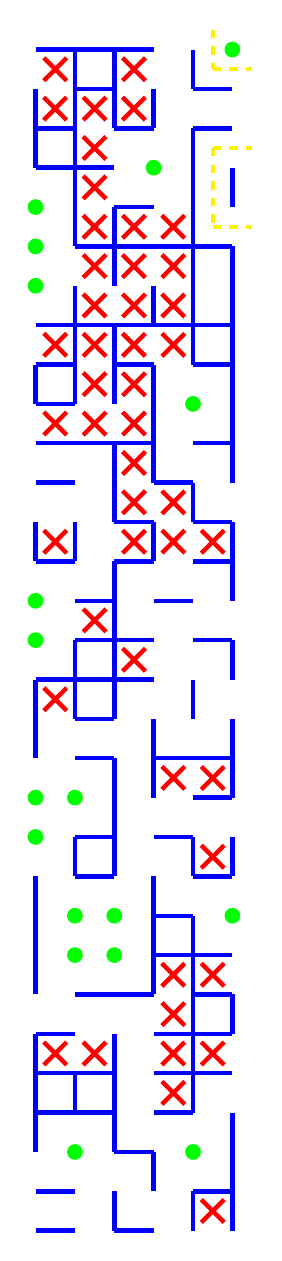
\begin{tikzpicture}[x=0.5cm, y=-0.5cm, ultra thick, blue]
% Walls
    \draw (0,0) -- (3,0);
    \draw (1,1) -- (2,1);
    \draw (4,1) -- (5,1);
    \draw (0,2) -- (1,2);
    \draw (2,2) -- (3,2);
    \draw (4,2) -- (5,2);
    \draw (0,3) -- (2,3);
    \draw (2,4) -- (3,4);
    \draw (1,5) -- (5,5);
    \draw (0,7) -- (5,7);
    \draw (0,8) -- (1,8);
    \draw (2,8) -- (3,8);
    \draw (4,8) -- (5,8);
    \draw (0,9) -- (1,9);
    \draw (0,10) -- (3,10);
    \draw (4,10) -- (5,10);
    \draw (0,11) -- (1,11);
    \draw (3,11) -- (4,11);
    \draw (2,12) -- (3,12);
    \draw (4,12) -- (5,12);
    \draw (0,13) -- (1,13);
    \draw (2,13) -- (3,13);
    \draw (4,13) -- (5,13);
    \draw (1,14) -- (2,14);
    \draw (3,14) -- (4,14);
    \draw (1,15) -- (3,15);
    \draw (4,15) -- (5,15);
    \draw (0,16) -- (3,16);
    \draw (1,17) -- (2,17);
    \draw (1,18) -- (2,18);
    \draw (3,18) -- (5,18);
    \draw (4,19) -- (5,19);
    \draw (1,20) -- (2,20);
    \draw (3,20) -- (4,20);
    \draw (1,21) -- (2,21);
    \draw (4,21) -- (5,21);
    \draw (3,22) -- (4,22);
    \draw (3,23) -- (5,23);
    \draw (1,24) -- (3,24);
    \draw (4,24) -- (5,24);
    \draw (0,25) -- (1,25);
    \draw (3,25) -- (5,25);
    \draw (0,26) -- (2,26);
    \draw (3,26) -- (5,26);
    \draw (0,27) -- (2,27);
    \draw (3,27) -- (4,27);
    \draw (2,28) -- (3,28);
    \draw (0,29) -- (1,29);
    \draw (4,29) -- (5,29);
    \draw (0,30) -- (1,30);
    \draw (2,30) -- (3,30);
    \draw (0,1) -- (0,3);
    \draw (0,8) -- (0,9);
    \draw (0,12) -- (0,13);
    \draw (0,16) -- (0,18);
    \draw (0,21) -- (0,24);
    \draw (0,25) -- (0,28);
    \draw (1,0) -- (1,5);
    \draw (1,6) -- (1,9);
    \draw (1,12) -- (1,13);
    \draw (1,15) -- (1,17);
    \draw (1,20) -- (1,21);
    \draw (1,26) -- (1,27);
    \draw (2,0) -- (2,2);
    \draw (2,4) -- (2,6);
    \draw (2,7) -- (2,9);
    \draw (2,10) -- (2,12);
    \draw (2,13) -- (2,17);
    \draw (2,18) -- (2,21);
    \draw (2,25) -- (2,28);
    \draw (2,29) -- (2,30);
    \draw (3,1) -- (3,2);
    \draw (3,6) -- (3,7);
    \draw (3,8) -- (3,11);
    \draw (3,12) -- (3,13);
    \draw (3,17) -- (3,19);
    \draw (3,21) -- (3,24);
    \draw (3,28) -- (3,29);
    \draw (4,0) -- (4,1);
    \draw (4,2) -- (4,8);
    \draw (4,11) -- (4,12);
    \draw (4,16) -- (4,17);
    \draw (4,20) -- (4,21);
    \draw (4,22) -- (4,27);
    \draw (4,29) -- (4,30);
    \draw (5,3) -- (5,4);
    \draw (5,5) -- (5,11);
    \draw (5,12) -- (5,14);
    \draw (5,15) -- (5,16);
    \draw (5,17) -- (5,19);
    \draw (5,20) -- (5,21);
    \draw (5,24) -- (5,25);
    \draw (5,27) -- (5,30);
% Pillars
    \fill[green] (5,0) circle(0.2);
    \fill[green] (3,3) circle(0.2);
    \fill[green] (0,4) circle(0.2);
    \fill[green] (0,5) circle(0.2);
    \fill[green] (0,6) circle(0.2);
    \fill[green] (4,9) circle(0.2);
    \fill[green] (0,14) circle(0.2);
    \fill[green] (0,15) circle(0.2);
    \fill[green] (0,19) circle(0.2);
    \fill[green] (1,19) circle(0.2);
    \fill[green] (0,20) circle(0.2);
    \fill[green] (1,22) circle(0.2);
    \fill[green] (2,22) circle(0.2);
    \fill[green] (5,22) circle(0.2);
    \fill[green] (1,23) circle(0.2);
    \fill[green] (2,23) circle(0.2);
    \fill[green] (1,28) circle(0.2);
    \fill[green] (4,28) circle(0.2);
% Inner points in accessible cul-de-sacs
    \node at (0.5,0.5) {};
    \node at (2.5,0.5) {};
    \node at (0.5,1.5) {};
    \node at (1.5,1.5) {};
    \node at (2.5,1.5) {};
    \node at (1.5,2.5) {};
    \node at (1.5,3.5) {};
    \node at (1.5,4.5) {};
    \node at (2.5,4.5) {};
    \node at (3.5,4.5) {};
    \node at (1.5,5.5) {};
    \node at (2.5,5.5) {};
    \node at (3.5,5.5) {};
    \node at (1.5,6.5) {};
    \node at (2.5,6.5) {};
    \node at (3.5,6.5) {};
    \node at (0.5,7.5) {};
    \node at (1.5,7.5) {};
    \node at (2.5,7.5) {};
    \node at (3.5,7.5) {};
    \node at (1.5,8.5) {};
    \node at (2.5,8.5) {};
    \node at (0.5,9.5) {};
    \node at (1.5,9.5) {};
    \node at (2.5,9.5) {};
    \node at (2.5,10.5) {};
    \node at (2.5,11.5) {};
    \node at (3.5,11.5) {};
    \node at (0.5,12.5) {};
    \node at (2.5,12.5) {};
    \node at (3.5,12.5) {};
    \node at (4.5,12.5) {};
    \node at (1.5,14.5) {};
    \node at (2.5,15.5) {};
    \node at (0.5,16.5) {};
    \node at (3.5,18.5) {};
    \node at (4.5,18.5) {};
    \node at (4.5,20.5) {};
    \node at (3.5,23.5) {};
    \node at (4.5,23.5) {};
    \node at (3.5,24.5) {};
    \node at (0.5,25.5) {};
    \node at (1.5,25.5) {};
    \node at (3.5,25.5) {};
    \node at (4.5,25.5) {};
    \node at (3.5,26.5) {};
    \node at (4.5,29.5) {};
% Entry-exit paths without intersections
    \draw[dashed, yellow] (4.5,0.5) -- (5.5,0.5);
    \draw[dashed, yellow] (4.5,2.5) -- (5.5,2.5);
    \draw[dashed, yellow] (4.5,4.5) -- (5.5,4.5);
    \draw[dashed, yellow] (4.5,-0.5) -- (4.5,0.5);
    \draw[dashed, yellow] (4.5,2.5) -- (4.5,4.5);
\end{tikzpicture}
\end{center}
\vspace*{\fill}

\end{document}
